\documentclass[a4paper,twoside,12pt,chapterprefix=false]{scrbook}

\usepackage{amsmath,amssymb,amsthm}
\usepackage[footnotesize,sl,SL,hang,tight]{subfigure}  % helpful package for aligning figures next to each other
\usepackage{longtable} % tables over several pages
\usepackage[font={small,sl},hang,labelfont=bf]{caption} % configure captions
%\usepackage{captcont} % continue sufigures over several pages
\usepackage{booktabs} % publication quality tables for LaTeX
%\usepackage{showkeys} % shows the labels above the references for easier development

\ifpdfoutput{%
	\usepackage[pdftex]{graphicx}
	\usepackage[]{pdfpages} %for including full pdf pages
}{%
	\usepackage{graphicx}
}
\usepackage{rotating} % rotate figures

\usepackage{scrpage2}
\KOMAoptions{headinclude}

% Font packages:
\usepackage{times}
\usepackage{helvet}   % sets sans serif font
\usepackage[T1]{fontenc}

%PDF hyperref config
\ifpdfoutput{%
	\usepackage[pdftex,
		bookmarks,
		bookmarksopen=true,
		bookmarksnumbered=true,
		pdfauthor={My Name},
		pdftitle={Thesis Title},
		colorlinks,
		linkcolor=black,
		citecolor=black,
		filecolor=black,
		urlcolor=black,
		anchorcolor=black,
		menucolor=black,
		breaklinks=true,
		pageanchor=true,
		plainpages=false,
		pdfpagelabels=true]{hyperref}
}{}

\ifpdfoutput{%
	\pdfcompresslevel=9
	\pdfoutput=1
	\DeclareGraphicsExtensions{.pdf,.png}
}{}

\bibliographystyle{alpha}

% Uncomment the chapter / section you are working on.
%
%\includeonly{figures}
%\includeonly{tables}
%\includeonly{data-analysis}
%\includeonly{conclusion}
%\includeonly{apx-sample-appendix}

%\pagestyle{useheadings}

% A4
%
\topmargin -0.5in
\textheight 9.3in
\textwidth 6.3in
\oddsidemargin 0.18in
\evensidemargin -0.22in
\parskip 0.1in
\parindent 0in

\renewcommand{\arraystretch}{1.5}
\renewcommand{\baselinestretch}{1}

% commands
\newcommand{\Adjoint}{\mbox{\rm Adj}}
\newcommand{\Area}{\mbox{\rm Area}}
\newcommand{\ACos}{{\mbox{\rm Cos}^{-1}}}
\newcommand{\ASin}{{\mbox{\rm Sin}^{-1}}}
\newcommand{\ATan}{{\mbox{\rm atan2}}}
\newcommand{\Code}[1]{{\tt #1}}
\newcommand{\Complex}{\mbox{\bf C}}
\newcommand{\Cross}{{\mbox{\rm Cross}}}
\newcommand{\Mydddot}[1]{\mbox{\shortstack{$.$\hspace*{-1pt}$.$\hspace*{-1pt}$.$\\$#1$}}}
\newcommand{\Degree}{\mbox{\rm degree}}
\newcommand{\Diag}{\mbox{\rm Diag}}
\newcommand{\Dim}{\mbox{\rm dim}}
\newcommand{\Dist}{\mbox{\rm Distance}}
\newcommand{\IntTwo}{\int\!\!\int}
\newcommand{\IntThree}{\int\!\!\int\! \!\int}
\newcommand{\Kernel}{\mbox{\rm kernel}}
\newcommand{\Kross}{\mbox{\rm Kross}}
\newcommand{\Grad}{\nabla}
\newcommand{\Perp}{\mbox{\rm Perp}}
\newcommand{\Point}[1]{{\cal #1}}
\newcommand{\Rank}{\mbox{\rm rank}}
\newcommand{\Range}{\mbox{\rm range}}
\newcommand{\Real}{{\mbox{\rm I}\hspace*{-2pt}\mbox{\rm R}}}
\newcommand{\RealSbt}{{\mbox{\rm\scriptsize I}\hspace*{-2pt}\mbox{\rm\scriptsize R}}}
\newcommand{\Res}{\mbox{\rm resultant}}
\newcommand{\Sbt}[1]{{\mbox{\rm\scriptsize #1}}}
\newcommand{\MySign}{\mbox{\rm Sign}}
\newcommand{\SignSBT}{\mbox{\rm\scriptsize Sign}}
\newcommand{\Skew}{\mbox{\rm Skew}}
\newcommand{\Span}{\mbox{\rm Span}}
\newcommand{\SqrDist}{\mbox{\rm Distance$^2$}}
\newcommand{\Trace}{\mbox{\rm Trace}}
\newcommand{\TRN}{{\mbox{\rm\scriptsize T}}}
\newcommand{\Vector}[1]{\mbox{\bf #1}}
\newcommand{\VectorM}[1]{\mbox{\boldmath $#1$}}
\newcommand{\Volume}{\mbox{\rm Volume}}

\newcommand{\IVec}{\mbox{\boldmath $\imath$}}
\newcommand{\JVec}{\mbox{\boldmath $\jmath$}}
\newcommand{\KVec}{\mbox{\boldmath $k$}}
\newcommand{\LVec}{\mbox{\boldmath $\ell$}}
\newcommand{\RMat}{{\cal R}}
\newcommand{\QMat}{{\cal Q}}
\newcommand{\QCMat}{\overline{\cal Q}}

\newcommand{\Lerp}{\mbox{\rm lerp}}
\newcommand{\Slerp}{\mbox{\rm slerp}}
\newcommand{\Quad}{\mbox{\rm quad}}
\newcommand{\Squad}{\mbox{\rm squad}}

\newcommand{\subsubsubsection}[1]{{\sc #1}}

\newcommand{\ODer}[2]{\frac{d #1}{d #2}}
\newcommand{\ODerT}[2]{\frac{d^2 #1}{d {#2}^2}}
\newcommand{\ODerM}[3]{\frac{d #1}{d #2 \, d #3}}
\newcommand{\PDer}[2]{\frac{\partial #1}{\partial #2}}
\newcommand{\PDerT}[2]{\frac{\partial^2 #1}{\partial {#2}^2}}
\newcommand{\PDerM}[3]{\frac{\partial^2 #1}{\partial #2 \, \partial #3}}

% mass density symbol
\newcommand{\Den}{\delta}

% environments
\newenvironment{BArray}[1]{\left\{ \begin{array}{#1}}{\end{array} \right\}}
\newenvironment{Combin}{\left( \begin{array}{c}}{\end{array} \right)}
\newenvironment{Matrix}[1]{\left[ \begin{array}{#1}}{\end{array} \right]}

% "Figure" environment
\newtheorem{localFigure}{Figure}[chapter]
\newenvironment{Figure}[1]{
  \begin{center}
  \begin{minipage}{6in}
  \par\noindent\hspace*{0pt}\hrulefill
  
  \begin{localFigure} \label{#1}
}{
  \end{localFigure}
  \par\noindent\hspace*{0pt}\hrulefill
  \end{minipage}
  \end{center}
}

% "Table" environment
\newtheorem{localTable}{Table}[chapter]
\newenvironment{Table}[1]{
  \begin{center}
  \begin{minipage}{6in}
  
  \begin{localTable} \label{#1}
}{
  \end{localTable}
  \end{minipage}
  \end{center}
}

% "CDROM" environment for source code on disk
%\newenvironment{CDROM}[1]{
%  \label{#1} 
%    \includegraphics{cdrom.png} \hspace*{0.1in}{\tt PointShop3D}. \rm
%}{
%  $\bowtie$
%}

% TO DO search symbol
\newcommand{\TODO}{\mbox{\large\bf TO DO}}
\newcommand{\REFR}{\mbox{\large\bf REFR}}

%  Terminates current page and paragraph, makes sure next page starts on
%  an odd-number, and generates a completely blank page, without page markers,
%  if necessary.
\newcommand{\clearemptydoublepage}{\newpage{\pagestyle{empty}\cleardoublepage}}

%%% Shoemake's commands
\DeclareMathOperator{\prp}{\text{\scshape perp}}
\DeclareMathOperator{\rot}{rot}
\DeclareMathOperator{\N}{N}
\providecommand{\vmag}[1]{\lVert#1\rVert}
\providecommand{\mutate}[1]{\overleftarrow{#1}}
\providecommand{\T}[1]{{#1}^{\mathrm T}}
\newcommand{\cross}{\times}
\newcommand{\by}{\times}
\newcommand{\vect}[1]{\mathbf{#1}}
\newcommand{\mat}[1]{\mathbf{#1}} % or not
%\newcommand{\quat}[1]{\mathbf{#1}}
\newcommand{\quat}[1]{\ensuremath{\mathbf{\dot{#1}}}}
\newcommand{\vV}{\vect{v}}
\newcommand{\vU}{\vect{u}}
\newcommand{\vE}{\vect{e}}
\newcommand{\vUh}{\hat{\vect{u}}}
\newcommand{\mQ}{\mat{Q}}
\newcommand{\mR}{\mat{R}}
\newcommand{\mM}{\mat{M}}
\newcommand{\mA}{\mat{A}}
\newcommand{\mB}{\mat{B}}
\newcommand{\mI}{\mat{I}}
\newcommand{\mJ}{\mat{J}}
\newcommand{\mX}{\mat{X}}
\newcommand{\mY}{\mat{Y}}
\newcommand{\mZ}{\mat{Z}}
\newcommand{\qo}{\quat{1}}
\newcommand{\qi}{\quat{i}}
\newcommand{\qj}{\quat{j}}
\newcommand{\qk}{\quat{k}}
\newcommand{\xh}{{x}}
\newcommand{\yh}{{y}}
\newcommand{\zh}{{z}}
\newcommand{\ch}{c}
\newcommand{\sh}{s}
\newcommand{\gt}{\theta}


%%
%%
%%


\begin{document}

%% Define leading chapter pages
%
%\addtokomafont{chapter}{\setlength{\parskip}{190pt}}   % SEVERE HACK to keep spacing to chapter art work
\renewcommand*{\chapterheadstartvskip}{\vspace*{215pt}}  % different hack to keep spacing to chapter artwork
%\addtokomafont{chapter}{\rmfamily}        % remove this if you prefer sans-serif section titles
%\addtokomafont{section}{\rmfamily}        % remove this if you prefer sans-serif section titles
%\addtokomafont{subsection}{\rmfamily}     % remove this if you prefer sans-serif section titles
%\addtokomafont{subsubsection}{\rmfamily}  % remove this if you prefer sans-serif section titles
%\addtokomafont{paragraph}{\rmfamily}      % replace by \sffamily if you prefer sans-serif para titles
\addtokomafont{paragraph}{\sffamily}

\def\mychpstyleintl{%
{\noindent\setlength{\tabcolsep}{0pt}\setlength{\arrayrulewidth}{2pt}%
\begin{tabular}{c}
\\[100pt]
\begin{tabular}{lr}
\begin{tabular}{p{0.6\linewidth}}
\\
\end{tabular}
&
\begin{tabular}{p{0.4\linewidth}}
\rightline{{%
\sffamily%
\fontseries{bx}%
\fontshape{n}%
\fontsize{100}{120}%choose baselineskip to be 1.2 times font size
\selectfont
\thechapter}}
\end{tabular}
\end{tabular}\\[300pt]
\end{tabular}
}}

\newpagestyle{mychapterpagestyle}{{\protect\mychpstyleintl}{\protect\mychpstyleintl}}{}
\newpagestyle{myappendixpagestyle}{{\protect\mychpstyleintl}{\protect\mychpstyleintl}}{}
%%

%% macros e.g.
\newcommand{\mfytext}[0]{my fancy text}

%refs
\newcommand{\chpref}[1]{Chapter \ref{#1}}
\newcommand{\secref}[1]{Section \ref{#1}}
%\newcommand{\equref}[1]{Equation \ref{#1}} %better use builtin \eqref{}
\newcommand{\figref}[1]{Figure \ref{#1}}
\newcommand{\tabref}[1]{Table \ref{#1}}
\newcommand{\apxref}[1]{Appendix \ref{#1}}
%%

\hypersetup{pageanchor=false} % disabling anchors for title page to avoid warning

%% Replace this by your own design of a title page
%
%\title{Thesis Title}
%\author{My Name}
%\date{September 2042}
%\maketitle
%\clearemptydoublepage
% --- selfmade version ----
\begin{titlepage}
	\topmargin 1.0cm
	\oddsidemargin 0.0cm
	\evensidemargin 0.0cm
	%\textwidth 6.5in
	\centering
	\Huge
	\vspace{3.0cm}
	\textbf{\textsf{Inferring Human Body Parts and Correlations from Images, Pointclouds and Meshes}} \\[2.0cm]
	%\includegraphics*[width=0.4\textwidth]{figures/titlefigure} \\[4.0cm]
	\vspace{5.0cm}
	\sffamily
	\Large
	David Haldimann
	\\[0.8cm]
	\large
	Semester Thesis
	\\
	June 2018
	\\[1.3cm]
	Prof. Dr. Markus Gross
	\vfill
	\includegraphics*[width=0.3\textwidth]{figures/ETH_logo} \hfill
	\includegraphics*[width=0.3\textwidth]{figures/CGL_logo}
	\vspace{3.4cm}
\end{titlepage}
\clearemptydoublepage
%%

\hypersetup{pageanchor=true}
\pagenumbering{roman}
\setcounter{page}{1}

\chapter*{Abstract}

This thesis addresses the development of a novel sample thesis. We analyze the requirements of a general template, as it can be used with the \LaTeX\ text processing system. (And so on\dots) The abstract should not exceed half a page in size!

\cleardoublepage
\chapter*{Zusammenfassung}

Diese Arbeit besch�ftigt sich mit der Entwicklung einer neuartigen Beispielausarbeitung. Wir untersuchen die Anforderungen, die sich f�r eine allgemeine Vorlage ergeben, die innerhalb der \LaTeX-Textverarbeitungsumgebung verwendet werden kann. (Und so weiter und so fort\dots) Die Zusammenfassung sollte nicht l�nger als eine halbe Textseite sein!


%include task description here:
\cleardoublepage
%\includegraphics[viewport=3cm 0cm 20cm 27.5cm]{task_description} %better use includepdf below!
%\includepdf{task_description}
\cleardoublepage

%include acknowledgment here:
%\include{acknowledgment}

\tableofcontents
\cleardoublepage

\addcontentsline{toc}{chapter}{List of Figures}
\listoffigures
\cleardoublepage

\addcontentsline{toc}{chapter}{List of Tables}
\listoftables
\cleardoublepage

\pagenumbering{arabic}
\renewcommand*{\chapterpagestyle}{mychapterpagestyle}
\renewcommand*{\chapterformat}{} % show chapter titles only (no numbers)
% \setchapterpreamble[o]{...}  unfortunately does not move the \chapter output downwards

% ---- MAIN PART ----

% set counter to n-1:
\setcounter{chapter}{0}

\chapter{Introduction}

The price for breast enhancement surgery was estimated to be \$3718 in 2017 according to the American Society of Plastic Surgery\footnote{https://www.plasticsurgery.org/cosmetic-procedures/breast-augmentation/cost}. Next to the financial aspects, there are also risks connected to undergoing surgery as well as not knowing exactly what the result will look like. Before commiting to this kind of operation, it should be possible to generate a preview of the outcome from a few images. This thesis aims to design a method that is able to predict a 3D model of the outcome by learning a mapping between parametric models. Additionally, the idea is explored, if it is possible to generate a parametric model from a character modelling software.

%https://www.plasticsurgery.org/cosmetic-procedures/breast-augmentation/cost



\section{Parametric Model}
A previous implementation by Biland \cite{Biland17} was used to create parametric models. A parametric model can describe all data that went into the model with its parameters. For example, the physical appearance of a person can be roughly described by their height, skin tone and hair color, where these three are the parameters of this parametric model. This is, of course, only an approximation as the accuracy of the description of the person would increase with more parameters. It is also possible, that one parameter influences multiple features. In the previous example, when the height of a person is raised, the length of the arms are also proportionally increased.

\section{Mapping}
A mapping between sets associates each element in the first set with one or more elements of the second set. An example for a simple mapping could be the numbers one to twenty-six as the first set and the letters of the alphabet as the second. In the case of two parametric models, the goal is to find a mapping that describes the relationship between the parameters of the first and second model. \\
This mapping can either be linear or non-linear. The difference between a linearity and a non-linearity can be described with a simple example. The time it takes to drive $10km$ in a car at $10\frac{km}{h}$ is $1h$. If the distance to drive is doubled to $20km$, so will the time it takes. That is, because distance to drive and time it requires are in a linear relationship. On the other hand, given that the braking distance while travelling with $10\frac{km}{h}$ is $1m$, the braking distance while travelling with $20\frac{km}{h}$ is $4m$. This is due to the fact, that speed and braking distance are related in a quadratic, non-linear, manner.

\section{Applications}
The applications for this method could be plenty. While the most obvious use for this implementation would be plastic surgery - creating 3D models from images of possible breast enhancements, it could also be used in oncology, to show affected patients what their body might look like after a mastectomy and even further, after a possible reconstruction. This approach could also be used in an adapted version for commercial use, such as tailor fitting clothes by using an image of the customer.

% set counter to n-1:
\setcounter{chapter}{1}

\chapter{Related Work}
In the field of modelling the human body, early on, a lot of work was done concerning the face. Jeng et al. \cite{jeng1998facial} proposed a geometric face model to localize the face in an image and detect facial features efficiently. The reason for the need of a functioning model for faces may have been the upcoming importance of faciel recognition.\\
Parametric models have also been applied to reshaping the human body in images using semantic parameters. \cite{zhou2010parametric} Their approach included reshaping a morphable 3D model and applying the reshaping effects using an image warping approach. Other work was done by Allen et al. \cite{allen2003space} on parametrizing full body scans and using the parameters in a variety of applications. One application was to find features connected to certain parameters, such that for example the weight could be increased and the resulting mesh would increase in size in a meaningful way.\\
Work about specifically modelling the breast has been done by Galle et al. \cite{gallo2010human}. They proposed a parameter space based on MRI scans to describe the shape of a human breast using PCA. Ciechomski et al. \cite{de2012development} proposed a web approach to create 3D models from images where participants uploaded images and selected keypoints. These 3D models can later be accessed by surgeons to visualize different types and sizes of implants applied.

\chapter{Your Central Work}

Lorem ipsum dolor sit amet, consectetuer adipiscing elit, sed diam nonummy nibh euismod tincidunt ut laoreet dolore magna aliquam erat volutpat. Ut wisi enim ad minim veniam, quis nostrud exerci tation ullamcorper suscipit lobortis nisl ut aliquip ex ea commodo consequat. Duis autem vel eum iriure dolor in hendrerit in vulputate velit esse molestie consequat, vel illum dolore eu feugiat nulla facilisis at vero et accumsan et iusto odio dignissim qui blandit.

\section{First Section}

Lorem ipsum dolor sit amet, consectetuer adipiscing elit, sed diam nonummy nibh euismod tincidunt ut laoreet dolore magna aliquam erat volutpat. Ut wisi enim ad minim veniam, quis nostrud exerci tation ullamcorper suscipit lobortis nisl ut aliquip ex ea commodo consequat. Duis autem vel eum iriure dolor in hendrerit in vulputate velit esse molestie consequat, vel illum dolore eu feugiat nulla facilisis at vero et accumsan et iusto odio dignissim qui blandit praesent luptatum zzril delenit augue duis dolore te feugait nulla facilisi. Lorem ipsum dolor sit amet, consectetuer adipiscing elit, sed diam  praesent luptatum zzril delenit augue duis dolore te feugait nulla facilisi. Lorem ipsum dolor sit amet, consectetuer adipiscing elit, sed diam nonummy nibh euismod tincidunt ut laoreet dolore magna aliquam erat volutpat. Ut wisi enim ad minim veniam, quis nostrud exerci tation ullamcorper suscipit lobortis nisl ut aliquip ex ea commodo consequat. Duis autem vel eum iriure dolor in hendrerit in vulputate velit esse molestie consequat, vel illum dolore eu feugiat nulla facilisis at vero et accumsan et iusto odio dignissim qui blandit.

Delenit augue duis dolore te feugait nulla facilisi. Lorem ipsum dolor sit amet, consectetuer adipiscing elit, sed diam  praesent luptatum zzril delenit augue duis dolore te feugait nulla facilisi. Lorem ipsum dolor sit amet, consectetuer adipiscing elit, sed diam nonummy nibh euismod tincidunt ut laoreet dolore magna aliquam erat volutpat. Ut wisi enim ad minim veniam, quis nostrud exerci tation ullamcorper suscipit lobortis nisl ut aliquip ex ea commodo consequat. Duis autem vel eum iriure dolor in hendrerit in vulputate velit esse molestie consequat, vel illum dolore eu feugiat nulla facilisis at vero et accumsan et iusto odio dignissim qui blandit.

\subsection{Fist Subsection}

Lorem ipsum dolor sit amet, consectetuer adipiscing elit, sed diam nonummy nibh euismod tincidunt ut laoreet dolore magna aliquam erat volutpat. Ut wisi enim ad minim veniam, quis nostrud exerci tation ullamcorper suscipit lobortis nisl ut aliquip ex ea commodo consequat. Duis autem vel eum iriure dolor in hendrerit in vulputate velit esse molestie consequat, vel illum dolore eu feugiat nulla facilisis at vero et accumsan et iusto odio dignissim qui blandit praesent luptatum zzril delenit augue duis dolore te feugait nulla facilisi. Lorem ipsum dolor sit amet, consectetuer adipiscing elit, sed diam 

\subsection{Another Subsection}

\begin{table}
    \centering
    \begin{tabular}{|l|p{0.4\linewidth}|}
    \hline
    \emph{Quant.} & \emph{Ingredient}\\
    \hline
		200g &Wei{\ss}mehl\\
		1/4  &Packung Frischhefe\\
		4EL  &lauwarme Milch\\
		4EL  &�l\\
		1TL  &Zucker\\
		1TL  &Salz\\
		&lauwarmes Wasser\\
    \hline
    \end{tabular}
    \caption[Flammkuchenteig]{Flammkuchenteig. The ingredients have to be carefully chosen.\label{tab:mytable}}
\end{table}
%
Lorem ipsum dolor sit amet, consectetuer adipiscing elit, sed diam nonummy nibh euismod tincidunt ut laoreet dolore magna aliquam erat volutpat. Ut wisi enim ad minim veniam, quis nostrud exerci tation ullamcorper suscipit lobortis nisl ut aliquip ex ea commodo consequat, see Table~\ref{tab:mytable}. Duis autem vel eum iriure dolor in hendrerit in vulputate velit esse molestie consequat, vel illum dolore eu feugiat nulla facilisis at vero et accumsan et iusto odio dignissim qui blandit praesent luptatum zzril delenit augue duis dolore te feugait nulla facilisi. Lorem ipsum dolor sit amet, consectetuer adipiscing elit, sed diam,
see Figure~\ref{fig:voldiff}~(a).
%
\begin{figure}
    \centering
    \setlength{\tabcolsep}{0.0130\linewidth}
    \begin{tabular}{@{}cc@{}}
    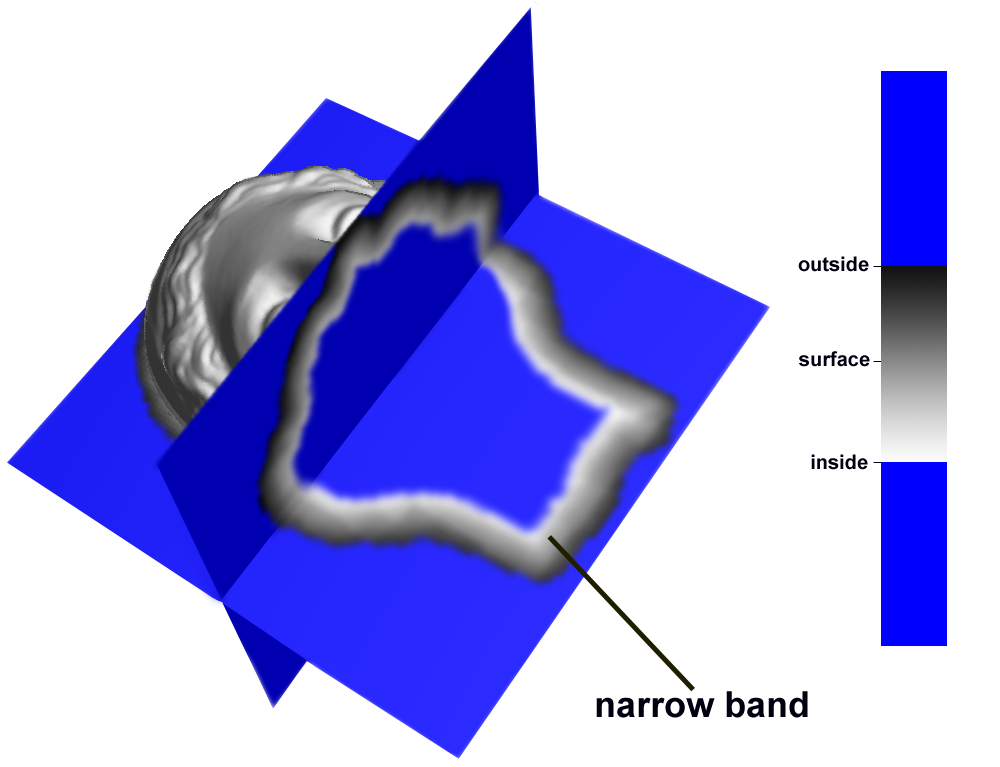
\includegraphics[width=0.487\linewidth]{figures/IgeaNarrowBand}&
    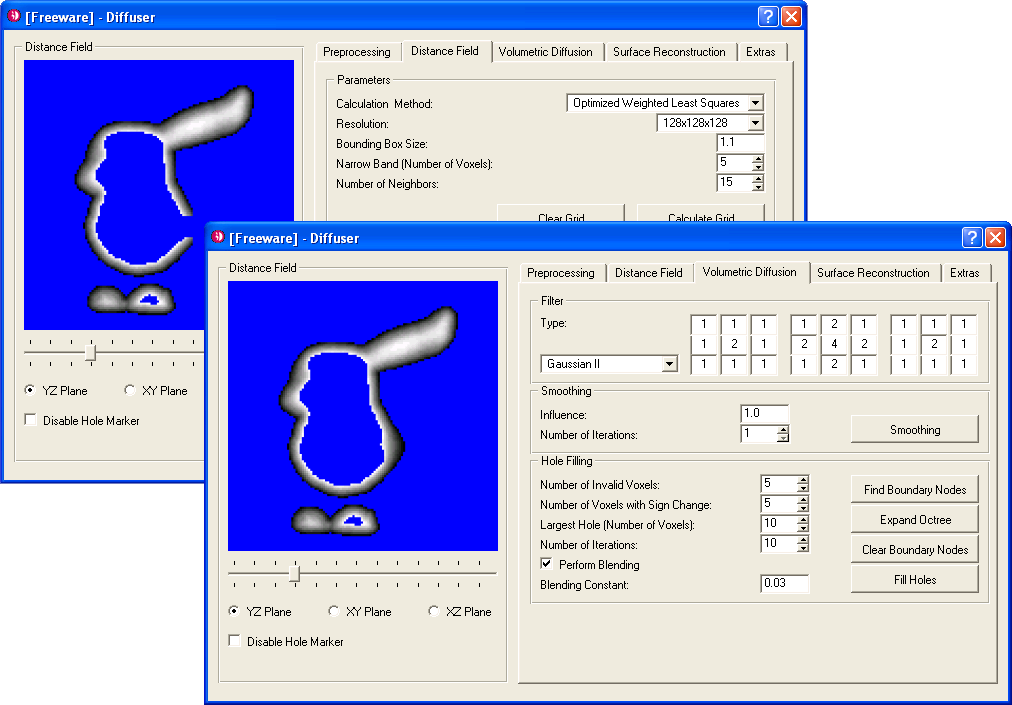
\includegraphics[width=0.487\linewidth]{figures/voldiff_ui}\\
    (a)&(b)\\
    \end{tabular}
    \caption[Volumetric diffusion]{Volumetric diffusion.
    	  \textup{(a)} Slices of the distance volume reveal the narrow band.
			  \textup{(b)} The user interface of the automatic hole filling
        tool allows to fine-tune the algorithm.
        The volumetric representation can be previewed before
        surface reconstruction.%
      \label{fig:voldiff}}
\end{figure}
%
Isn't it?

\begin{figure}[!htb]
	\centering
	\subfigure[Caption first.]{\label{fig:test1}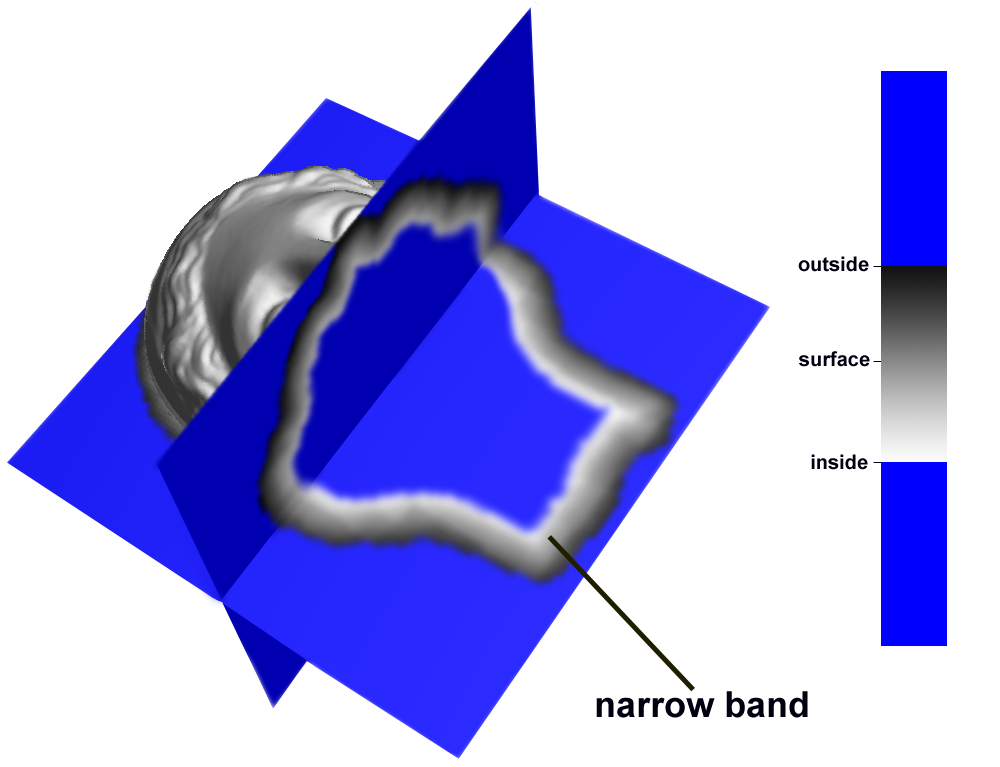
\includegraphics[width=0.3\textwidth]{figures/IgeaNarrowBand}} \hfill
	\subfigure[Caption second.]{\label{fig:test2}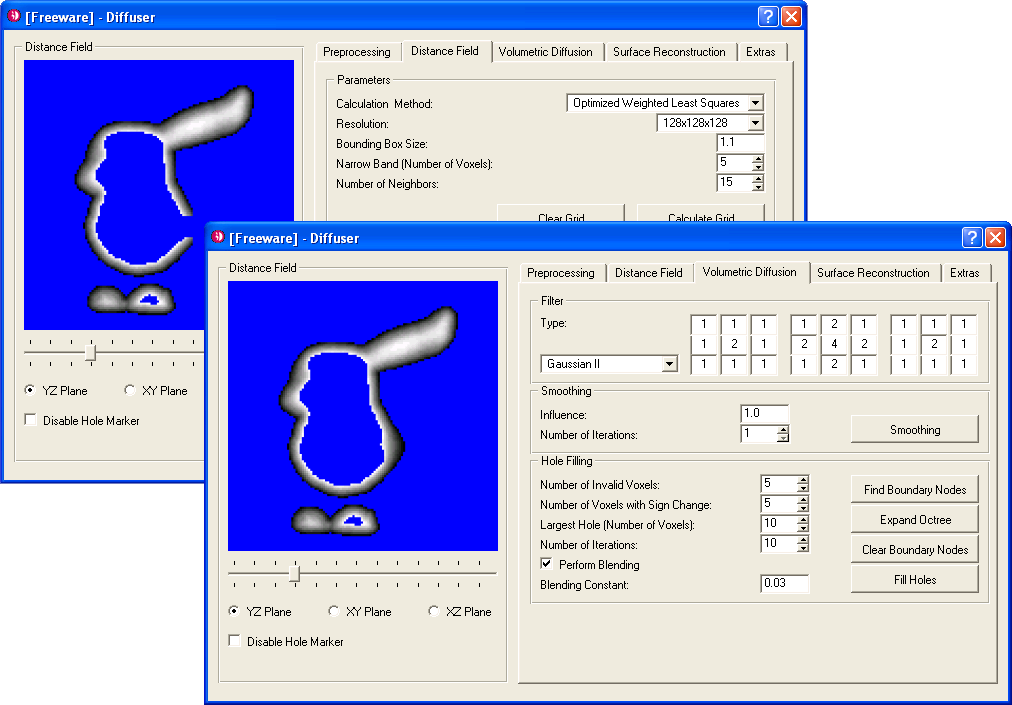
\includegraphics[width=0.3\textwidth]{figures/voldiff_ui}}
	\caption[Caption both]{Caption of both \subref{fig:test1}, \subref{fig:test2}.}
	\label{fig:bothfigures}
\end{figure}


Lorem ipsum dolor sit amet, consectetuer adipiscing elit, sed diam nonummy nibh euismod tincidunt ut laoreet dolore magna aliquam erat volutpat. Ut wisi enim ad minim veniam, quis nostrud exerci tation ullamcorper suscipit lobortis nisl ut aliquip ex ea commodo consequat. Duis autem vel eum iriure dolor in hendrerit in vulputate velit esse molestie consequat, vel illum dolore eu feugiat nulla facilisis at vero et accumsan et iusto odio dignissim qui blandit praesent luptatum zzril delenit augue duis dolore te feugait nulla facilisi. Lorem ipsum dolor sit amet, consectetuer adipiscing elit, sed diam 

\section{Second Section}

Lorem ipsum dolor sit amet, consectetuer adipiscing elit, sed diam nonummy nibh euismod tincidunt ut laoreet dolore magna aliquam erat volutpat. Ut wisi enim ad minim veniam, quis nostrud exerci tation ullamcorper suscipit lobortis nisl ut aliquip ex ea commodo consequat. Duis autem vel eum iriure dolor in hendrerit in vulputate velit esse molestie consequat, vel illum dolore eu feugiat nulla facilisis at vero et accumsan et iusto odio dignissim qui blandit praesent luptatum zzril delenit augue duis dolore te feugait nulla facilisi. Lorem ipsum dolor sit amet, consectetuer adipiscing elit, sed diam nonummy nibh euismod tincidunt ut laoreet dolore magna aliquam erat volutpat. Ut wisi enim ad minim veniam, quis nostrud exerci tation ullamcorper suscipit lobortis nisl ut aliquip ex ea commodo consequat. Duis autem vel eum iriure dolor in hendrerit in vulputate velit esse molestie consequat, vel illum dolore eu feugiat nulla facilisis at vero et accumsan et iusto odio dignissim qui blandit

\chapter{Conclusion and Outlook}

Lorem ipsum dolor sit amet, consectetuer adipiscing elit, sed diam nonummy nibh euismod tincidunt ut laoreet dolore magna aliquam erat volutpat. Ut wisi enim ad minim veniam, quis nostrud exerci tation ullamcorper suscipit lobortis nisl ut aliquip ex ea commodo consequat. Duis autem vel eum iriure dolor in hendrerit in vulputate velit esse molestie consequat, vel illum dolore eu feugiat nulla facilisis at vero et accumsan et iusto odio dignissim qui blandit praesent luptatum zzril delenit augue duis dolore te feugait nulla facilisi. Lorem ipsum dolor sit amet, consectetuer adipiscing elit, sed diam nonummy nibh euismod tincidunt ut laoreet dolore magna aliquam erat volutpat. Ut wisi enim ad minim veniam, quis nostrud exerci tation ullamcorper suscipit lobortis nisl ut aliquip ex ea commodo consequat. Duis autem vel eum iriure dolor in hendrerit in vulputate velit esse molestie consequat, vel illum dolore eu feugiat nulla facilisis at vero et accumsan et iusto odio dignissim qui blandit

Lorem ipsum dolor sit amet, consectetuer adipiscing elit, sed diam nonummy nibh euismod tincidunt ut laoreet dolore magna aliquam erat volutpat. Ut wisi enim ad minim veniam, quis nostrud exerci tation ullamcorper suscipit lobortis nisl ut aliquip ex ea commodo consequat. Duis autem vel eum iriure dolor in hendrerit in vulputate velit esse molestie consequat, vel illum dolore eu feugiat nulla facilisis at vero et accumsan et iusto odio dignissim qui blandit praesent luptatum zzril delenit augue duis dolore te feugait nulla facilisi. Lorem ipsum dolor sit amet, consectetuer adipiscing elit, sed diam nonummy nibh euismod tincidunt ut laoreet dolore magna aliquam erat volutpat. Ut wisi enim ad minim veniam, quis nostrud exerci tation ullamcorper suscipit lobortis nisl ut aliquip ex ea commodo consequat. Duis autem vel eum iriure dolor in hendrerit in vulputate velit esse molestie consequat, vel illum dolore eu feugiat nulla facilisis at vero et accumsan et iusto odio dignissim qui blandit
Lorem ipsum dolor sit amet, consectetuer adipiscing elit, sed diam nonummy nibh euismod tincidunt ut laoreet dolore magna aliquam erat volutpat. Ut wisi enim ad minim veniam, quis nostrud exerci tation ullamcorper suscipit lobortis nisl ut aliquip ex ea commodo consequat. Duis autem vel eum iriure dolor in hendrerit in vulputate velit esse molestie consequat, vel illum dolore eu feugiat nulla facilisis at vero et accumsan et iusto odio dignissim qui blandit praesent luptatum zzril delenit augue duis dolore te feugait nulla facilisi. Lorem ipsum dolor sit amet, consectetuer adipiscing elit, sed diam nonummy nibh euismod tincidunt ut laoreet dolore magna aliquam erat volutpat. Ut wisi enim ad minim veniam, quis nostrud exerci tation ullamcorper suscipit lobortis nisl ut aliquip ex ea commodo consequat. Duis autem vel eum iriure dolor in hendrerit in vulputate velit esse molestie consequat, vel illum dolore eu feugiat nulla facilisis at vero et accumsan et iusto odio dignissim qui blandit

Lorem ipsum dolor sit amet, consectetuer adipiscing elit, sed diam nonummy nibh euismod tincidunt ut laoreet dolore magna aliquam erat volutpat. Ut wisi enim ad minim veniam, quis nostrud exerci tation ullamcorper suscipit lobortis nisl ut aliquip ex ea commodo consequat. Duis autem vel eum iriure dolor in hendrerit in vulputate velit esse molestie consequat, vel illum dolore eu feugiat nulla facilisis at vero et accumsan et iusto odio dignissim qui blandit praesent luptatum zzril delenit augue duis dolore te feugait nulla facilisi. Lorem ipsum dolor sit amet, consectetuer adipiscing elit, sed diam nonummy nibh euismod tincidunt ut laoreet dolore magna aliquam erat volutpat. Ut wisi enim ad minim veniam, quis nostrud exerci tation ullamcorper suscipit lobortis nisl ut aliquip ex ea commodo consequat. Duis autem vel eum iriure dolor in hendrerit in vulputate velit esse molestie consequat, vel illum dolore eu feugiat nulla facilisis at vero et accumsan et iusto odio dignissim qui blandit



% ---- END MAIN PART ----


\appendix
\clearpage
\renewcommand*{\chapterpagestyle}{myappendixpagestyle}

\chapter{Appendix}

\begin{table}[]
\centering
\begin{tabular}{lllc}
\cline{2-4}
\multicolumn{1}{l|}{\textbf{PCA}}        & \multicolumn{1}{l|}{\textbf{Method}}        & \multicolumn{1}{l|}{\textbf{Possible Parameters}}                                                                                                           & \multicolumn{1}{c|}{\textbf{Best}} \\ \cline{2-4}
\multicolumn{1}{l|}{\textbf{Incomplete}} & \multicolumn{1}{l|}{\textbf{Random Forest}} & \multicolumn{1}{l|}{'estimator\_\_n\_estimators':{[}5,10,20,30{]},}                                                                                         & \multicolumn{1}{c|}{30}            \\ \cline{2-4}
\multicolumn{1}{l|}{\textbf{}}           & \multicolumn{1}{l|}{\textbf{}}              & \multicolumn{1}{l|}{\begin{tabular}[c]{@{}l@{}}'estimator\_\_max\_features':\\ ('auto', 'sqrt','log2'),\end{tabular}}                                       & \multicolumn{1}{c|}{auto}          \\ \cline{2-4}
\multicolumn{1}{l|}{\textbf{}}           & \multicolumn{1}{l|}{\textbf{}}              & \multicolumn{1}{l|}{'estimator\_\_max\_depth':{[}2,4,8,16{]}}                                                                                               & \multicolumn{1}{c|}{8}             \\ \cline{2-4}
\multicolumn{1}{l|}{\textbf{}}           & \multicolumn{1}{l|}{\textbf{DT}}            & \multicolumn{1}{l|}{'estimator\_\_criterion':('mse','friedman\_mse','mae'),}                                                                                & \multicolumn{1}{c|}{mse}           \\ \cline{2-4}
\multicolumn{1}{l|}{\textbf{}}           & \multicolumn{1}{l|}{\textbf{}}              & \multicolumn{1}{l|}{'estimator\_\_splitter':('random','best'),}                                                                                             & \multicolumn{1}{c|}{best}          \\ \cline{2-4}
\multicolumn{1}{l|}{\textbf{}}           & \multicolumn{1}{l|}{\textbf{}}              & \multicolumn{1}{l|}{'estimator\_\_max\_features':('auto', 'sqrt','log2'),}                                                                                  & \multicolumn{1}{c|}{auto}          \\ \cline{2-4}
\multicolumn{1}{l|}{\textbf{}}           & \multicolumn{1}{l|}{\textbf{}}              & \multicolumn{1}{l|}{'estimator\_\_max\_depth':{[}2,4,8,16{]}}                                                                                               & \multicolumn{1}{c|}{2}             \\ \cline{2-4}
\multicolumn{1}{l|}{\textbf{}}           & \multicolumn{1}{l|}{\textbf{MLP}}           & \multicolumn{1}{l|}{'estimator\_\_activation':('identity','tanh','logistic'),}                                                                              & \multicolumn{1}{c|}{identity}      \\ \cline{2-4}
\multicolumn{1}{l|}{\textbf{}}           & \multicolumn{1}{l|}{\textbf{}}              & \multicolumn{1}{l|}{'estimator\_\_solver':('lbfgs','adam','sgd'),}                                                                                          & \multicolumn{1}{c|}{sgd}           \\ \cline{2-4}
\multicolumn{1}{l|}{\textbf{}}           & \multicolumn{1}{l|}{\textbf{}}              & \multicolumn{1}{l|}{\begin{tabular}[c]{@{}l@{}}'estimator\_\_hidden\_layer\_sizes':\\ {[}(15,),(30,),(45,),(60,),(45,30,),(60,45,){]},\end{tabular}}        & \multicolumn{1}{c|}{(60,45,)}      \\ \cline{2-4}
\multicolumn{1}{l|}{\textbf{}}           & \multicolumn{1}{l|}{\textbf{MLPrelu}}       & \multicolumn{1}{l|}{'estimator\_\_activation':( 'relu'),}                                                                                                   & \multicolumn{1}{c|}{relu}          \\ \cline{2-4}
\multicolumn{1}{l|}{\textbf{}}           & \multicolumn{1}{l|}{\textbf{}}              & \multicolumn{1}{l|}{'estimator\_\_solver':('lbfgs','adam','sgd'),}                                                                                          & \multicolumn{1}{c|}{adam}          \\ \cline{2-4}
\multicolumn{1}{l|}{\textbf{}}           & \multicolumn{1}{l|}{\textbf{}}              & \multicolumn{1}{l|}{\begin{tabular}[c]{@{}l@{}}'estimator\_\_hidden\_layer\_sizes':\\ {[}(15,45,),(45,30,),(60,45,),(60,45,30),(60,45,15){]},\end{tabular}} & \multicolumn{1}{c|}{(45,30,)}      \\ \cline{2-4}
\multicolumn{1}{l|}{\textbf{}}           & \multicolumn{1}{l|}{\textbf{}}              & \multicolumn{1}{l|}{early\_stopping: true}                                                                                                                  & \multicolumn{1}{c|}{true}          \\ \cline{2-4}
\multicolumn{1}{l|}{\textbf{Complete}}   & \multicolumn{1}{l|}{\textbf{RF}}            & \multicolumn{1}{l|}{'estimator\_\_n\_estimators':{[}5,10,20,30{]},}                                                                                         & \multicolumn{1}{c|}{30}            \\ \cline{2-4}
\multicolumn{1}{l|}{\textbf{}}           & \multicolumn{1}{l|}{\textbf{}}              & \multicolumn{1}{l|}{'estimator\_\_max\_features':('auto', 'sqrt','log2'),}                                                                                  & \multicolumn{1}{c|}{auto}          \\ \cline{2-4}
\multicolumn{1}{l|}{\textbf{}}           & \multicolumn{1}{l|}{\textbf{}}              & \multicolumn{1}{l|}{'estimator\_\_max\_depth':{[}2,4,8,16{]}}                                                                                               & \multicolumn{1}{c|}{4}             \\ \cline{2-4}
\multicolumn{1}{l|}{\textbf{}}           & \multicolumn{1}{l|}{\textbf{DT}}            & \multicolumn{1}{l|}{'estimator\_\_criterion':('mse','friedman\_mse','mae'),}                                                                                & \multicolumn{1}{c|}{friedman\_mse} \\ \cline{2-4}
\multicolumn{1}{l|}{\textbf{}}           & \multicolumn{1}{l|}{\textbf{}}              & \multicolumn{1}{l|}{'estimator\_\_splitter':('random','best'),}                                                                                             & \multicolumn{1}{c|}{best}          \\ \cline{2-4}
\multicolumn{1}{l|}{\textbf{}}           & \multicolumn{1}{l|}{\textbf{}}              & \multicolumn{1}{l|}{'estimator\_\_max\_features':('auto', 'sqrt','log2'),}                                                                                  & \multicolumn{1}{c|}{auto}          \\ \cline{2-4}
\multicolumn{1}{l|}{\textbf{}}           & \multicolumn{1}{l|}{\textbf{}}              & \multicolumn{1}{l|}{'estimator\_\_max\_depth':{[}2,4,8,16{]}}                                                                                               & \multicolumn{1}{c|}{2}             \\ \cline{2-4}
\multicolumn{1}{l|}{\textbf{}}           & \multicolumn{1}{l|}{\textbf{MLP}}           & \multicolumn{1}{l|}{'estimator\_\_activation':('identity','tanh','logistic'),}                                                                              & \multicolumn{1}{c|}{tanh}          \\ \cline{2-4}
\multicolumn{1}{l|}{\textbf{}}           & \multicolumn{1}{l|}{\textbf{}}              & \multicolumn{1}{l|}{'estimator\_\_solver':('lbfgs','adam','sgd'),}                                                                                          & \multicolumn{1}{c|}{sgd}           \\ \cline{2-4}
\multicolumn{1}{l|}{\textbf{}}           & \multicolumn{1}{l|}{\textbf{}}              & \multicolumn{1}{l|}{\begin{tabular}[c]{@{}l@{}}'estimator\_\_hidden\_layer\_sizes':\\ {[}(15,),(30,),(45,),(60,),(45,30,),(60,45,){]},\end{tabular}}        & \multicolumn{1}{c|}{(60,45,)}      \\ \cline{2-4}
\multicolumn{1}{l|}{\textbf{}}           & \multicolumn{1}{l|}{\textbf{MLPrelu}}       & \multicolumn{1}{l|}{'estimator\_\_activation':( 'relu'),}                                                                                                   & \multicolumn{1}{c|}{relu}          \\ \cline{2-4}
\multicolumn{1}{l|}{\textbf{}}           & \multicolumn{1}{l|}{\textbf{}}              & \multicolumn{1}{l|}{'estimator\_\_solver':('lbfgs','adam','sgd'),}                                                                                          & \multicolumn{1}{c|}{sgd}           \\ \cline{2-4}
\multicolumn{1}{l|}{\textbf{}}           & \multicolumn{1}{l|}{\textbf{}}              & \multicolumn{1}{l|}{\begin{tabular}[c]{@{}l@{}}'estimator\_\_hidden\_layer\_sizes':\\ {[}(15,45,),(45,30,),(60,45,),(60,45,30),(60,45,15){]},\end{tabular}} & \multicolumn{1}{c|}{(60,45,30,)}   \\ \cline{2-4}
\multicolumn{1}{l|}{\textbf{}}           & \multicolumn{1}{l|}{\textbf{}}              & \multicolumn{1}{l|}{early\_stopping: true}                                                                                                                  & \multicolumn{1}{c|}{true}          \\ \cline{2-4}
                                         &                                             &                                                                                                                                                             & \multicolumn{1}{l}{}
\end{tabular}
\caption[Grid Search parameter table]{The possible parameters were varied to find the best combination. The best option can be seen in the last column.}
\label{gstable}

\end{table}


\clearpage
\renewcommand*{\chapterpagestyle}{empty}

%\nocite{*}
\addcontentsline{toc}{chapter}{Bibliography}
\bibliography{graphics}

\end{document}
